% !TEX root = ../thesis.tex

\chapter{Auswertung}
\label{ch:auswertung}

Zur Evaluation der Pipeline wurden verschiedene Teile rekonstruiert und die Ergebnisse mit vorhandenen CAD-Modellen verglichen.
Als Qualitätsmetrik wurde die Cloud-Mesh-Distanz zwischen Rekonstruktion und Ground Truth gewählt.
Dabei wird die durchschnittliche Distanz zwischen Vertices und den nächsten Faces des Vergleichobjekts betrachtet.


%\begin{figure}[H]
%	\centering
%	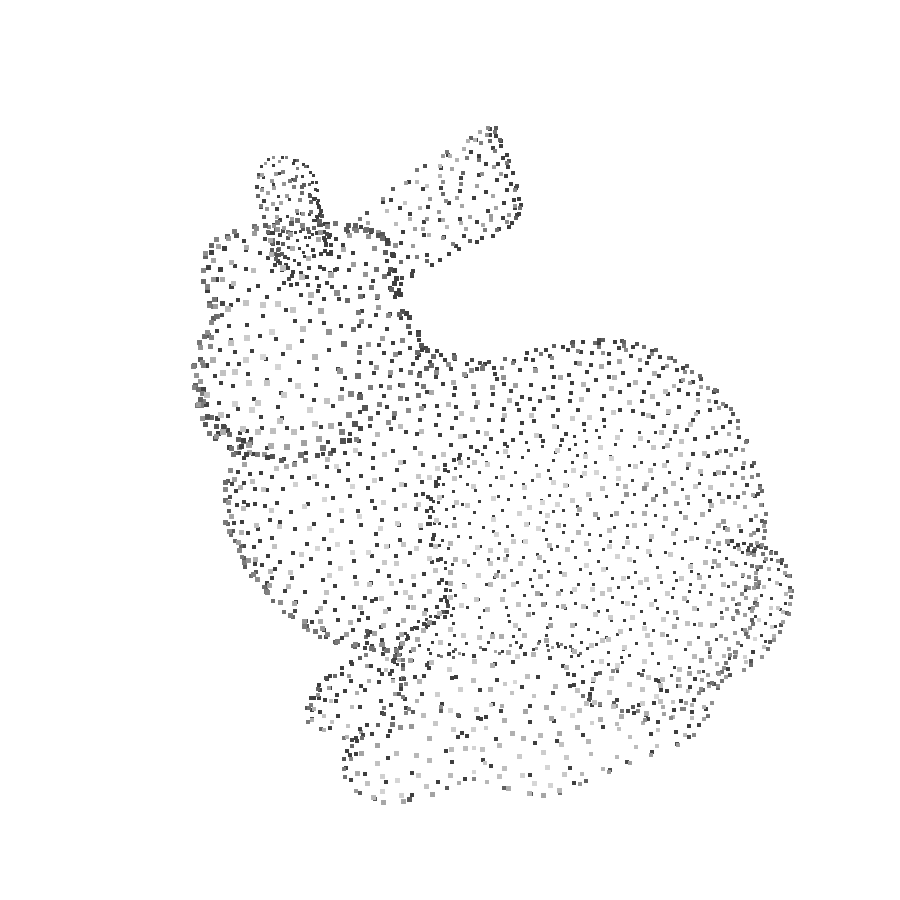
\includegraphics[width=0.33\textwidth, frame]{images/bunny_pcd.png}
%	\hspace{0.5cm}
%	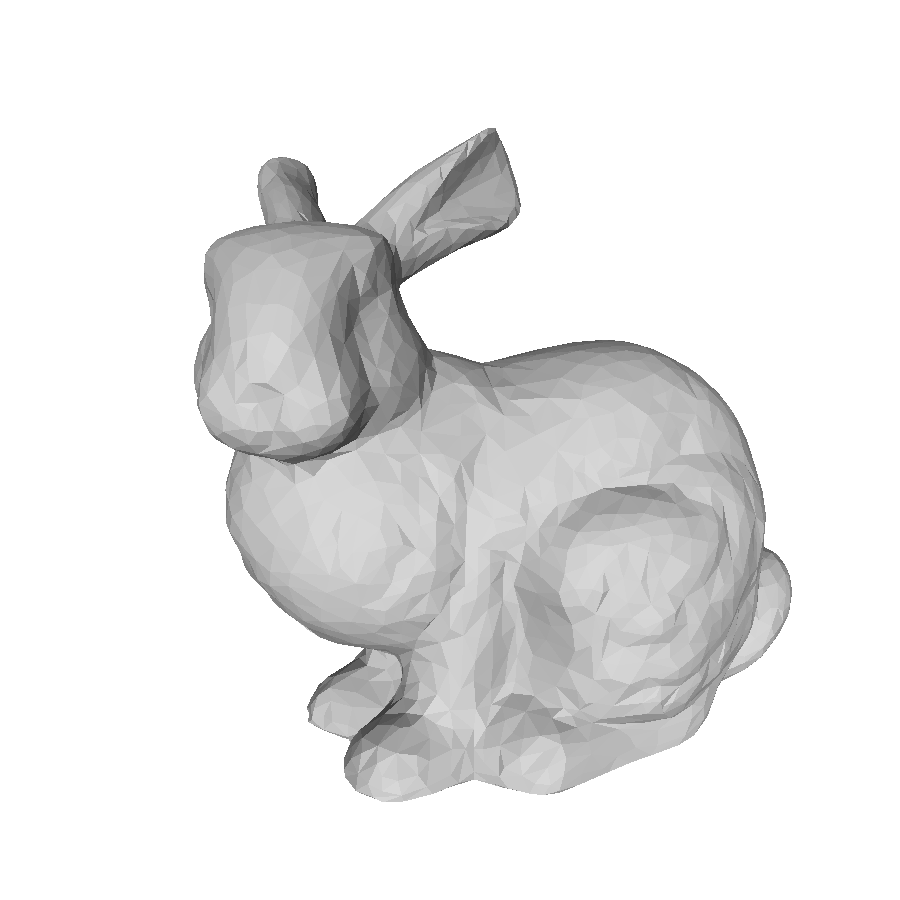
\includegraphics[width=0.33\textwidth, frame]{images/bunny_mesh.png}\\[0.5cm]
%	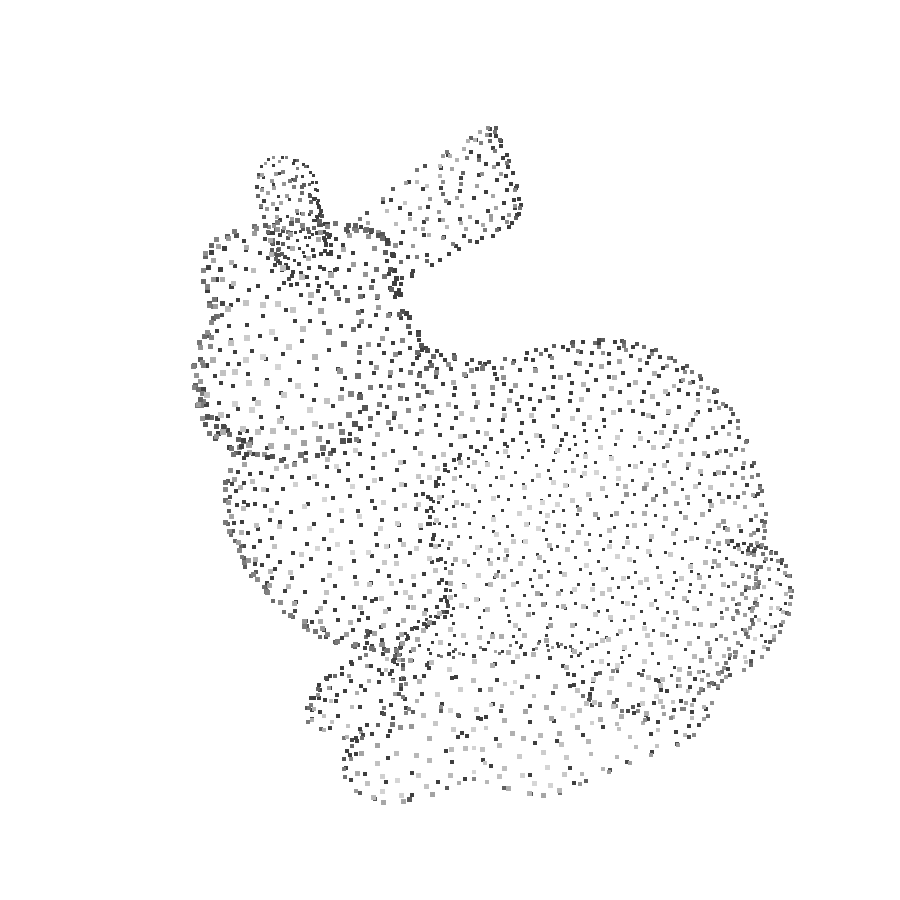
\includegraphics[width=0.33\textwidth, frame]{images/bunny_pcd.png}
%	\hspace{0.5cm}
%	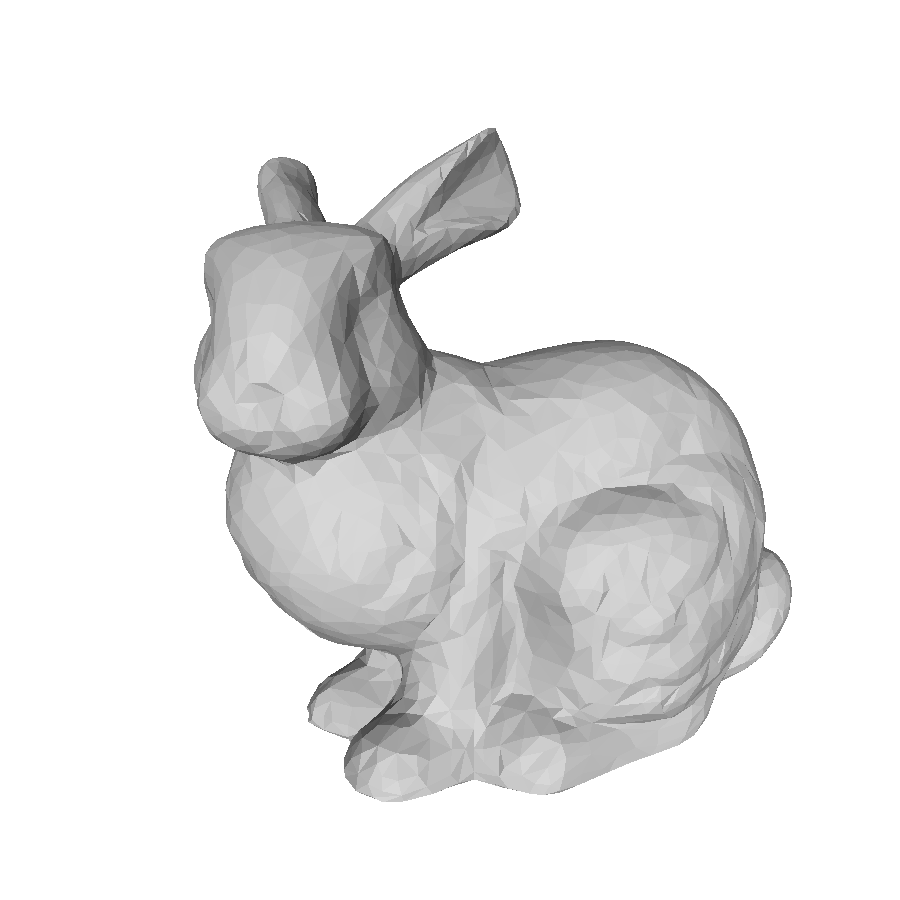
\includegraphics[width=0.33\textwidth, frame]{images/bunny_mesh.png}
%	\caption{Test image}
%	\label{fig:test}
%\end{figure}
%TODO